\chapter{Introduction to Linear Algebra}\label{chap:linear}

In this first chapter, we want to introduce all the major players in the linear arena. Linear Algebra is the study of \emph{linear} objects (a term we are not quite ready to define). As we have seen linear objects already many times in algebra and calculus, Linear Algebra will take a detailed look at linear structures and this first chapter will explore the important fundamentals of the linear universe.\\

Please be aware that this first chapter may feel awkward or difficult when you read it for the first time. This is both expected and intentional. If you were familiar with all the ideas behind Linear Algebra then you probably would not be reading this book. The struggle herein will produce questions, all of which we will answer in later chapters. Consider this chapter your baptism by fire into all things linear.


\begin{center}
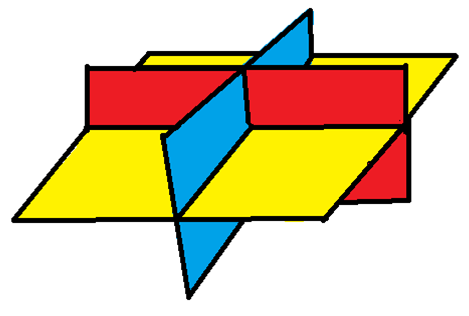
\includegraphics[scale=1]{Chapter1/images/Chapter1cover.png}%Kalvin Mudrow
\end{center}
%{\vspace{-10 pt}\hfill\footnotesize (Image contributed by Kalvin Mudrow)}\\ 

\pagebreak